\documentclass{article}
\usepackage[margin=2.5cm, top=4cm, headheight=25pt]{geometry}
\usepackage{amsmath, amssymb, enumitem, fancyhdr, graphicx}
\usepackage[indent=20pt]{parskip}
\usepackage[hidelinks]{hyperref}
\usepackage{xcolor}
\usepackage{listings}
\usepackage{subcaption}
\usepackage{url}
\usepackage[most]{tcolorbox}
\usepackage{lastpage}
\usepackage{tikz}
\usepackage{circuitikz}

\usetikzlibrary{arrows, positioning}
\tcbuselibrary{listingsutf8} % Support for lstlistings within tcolorbox

\newtcolorbox[auto counter, number within=section]{question}[1][]{%
    colframe=gray!80,                      % Dark gray frame
    colback=gray!5,                       % Light gray background
    coltitle=black,                        % Black title
    title=\textbf{Question~\thetcbcounter}, % Bold title
    fonttitle=\bfseries\large,             % Subtle title font size
    rounded corners,                   % Slightly more rounded corners
    boxrule=0.25mm,                         % Thinner border for a sleek look
    enhanced,                              % Enhanced box features
    attach boxed title to top left={xshift=2mm, yshift=-2mm},
    boxed title style={colframe=gray!80, colback=gray!5, boxrule=0.25mm},
    % Title styling
    #1
}

\bibliographystyle{IEEEtran}
\graphicspath{{./images/}}

% -- Custom Variables --
\def\me{Rajdeep Gill 7934493}
\def\course{ECE 3760}
\def\labsection{A01}

\def\labno{12}
\def\title{Assignment 12: H-Bridge}
% -- Styling for code snippets --
\lstset{
    basicstyle=\ttfamily\scriptsize,           % Basic font style
    keywordstyle=\color{blue},            % Keywords color
    commentstyle=\color{gray},            % Comments color
    stringstyle=\color{teal},             % Strings color
    numbers=left,                         % Line numbers on the left
    numberstyle=\tiny\color{gray},        % Line number style
    stepnumber=1,                         % Line number step
    numbersep=10pt,                       % Space between line numbers and code
    backgroundcolor=\color{lightgray!10}, % Background color
    frame=single,                         % Adds a frame around the code
    breaklines=true,                      % Line breaking for long lines
    captionpos=b,                         % Caption position
    showspaces=false,                     % Don't show spaces
    showstringspaces=false                % Don't show spaces in strings
}
\renewcommand{\lstlistingname}{Code Snippet}

\renewcommand{\arraystretch}{1.2} % For less-ugly tables
\setlength\parindent{0pt}

%----- Samples 
% Questions:
%   \begin{question}[title=Custom Question Title]
%       Question details
%   \end{question}

% Tables:
%   \begin{table}[htbp]
%       \centering
%       \caption{Table Caption}
%       \begin{tabular}{ll}
%           \toprule
%           \textbf{Column 1} & \textbf{Column 2} \\
%           \midrule
%           Row 1 & Row 2 \\
%           Row 3 & Row 4 \\
%           \bottomrule
%       \end{tabular}
%   \end{table} 

% Figures:
%   Single figure:
%       \begin{figure}[htbp]
%           \centering
%           \includegraphics[width=0.5\textwidth]{example-image}
%           \caption{Figure Caption}
%       \end{figure}
%   Multiple figures:
%       \begin{figure}[htbp]
%           \centering
%           \begin{subfigure}[b]{0.5\textwidth}
%               \includegraphics[width=\textwidth]{example-image-a}
%               \caption{First subfigure}
%           \end{subfigure}
%           \begin{subfigure}[b]{0.5\textwidth}
%               \includegraphics[width=\textwidth]{example-image-b}
%               \caption{Second subfigure}
%           \end{subfigure}
%           \caption{Main figure}
%       \end{figure}

\begin{document}

% --------------------------------------------------------------------------------
% TITLE
% --------------------------------------------------------------------------------

\begin{center}
    \huge \title

    \vspace{2mm}
    \hrule

    \vspace{4mm}
    \large \me

    \vspace{2mm}
    \large \course~\labsection

    \vspace{2mm}
    \today
\end{center}

\vspace{4mm}

% --------------------------------------------------------------------------------
% END TITLE
% --------------------------------------------------------------------------------

\newpage


\vspace{1cm}
\newpage

\pagestyle{fancy}
\fancyhead[L]{\large Assignment \labno}
\fancyhead[R]{\large \me}

\fancyfoot[C]{Page \thepage~of~\pageref{LastPage}}

% --------------------------------------------------------------------------------
% BODY
% --------------------------------------------------------------------------------
\section{H-Bridge}

\autoref{fig:labeled_diagram} showcases the labeled diagram of the H-Bridge circuit. At the top we have our power supply, Vdd, and the top two MOSFETs are P-type, while the bottom two are N-type. To make the motor spin in on direction, we turn on the top left and bottom right MOSFETs, while to reverse the direction we turn on the top right and bottom left MOSFETs, keeping the other two MOSFETs off.

\begin{figure}[ht!]
    \centering
    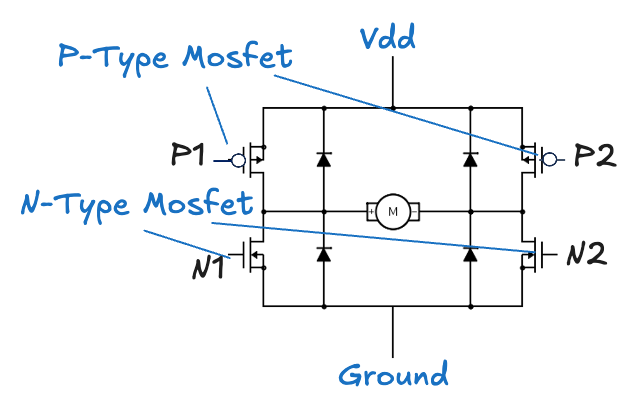
\includegraphics[width=0.75\textwidth]{labeled_h_bridge.png}
    \caption{Labeled diagram of H-Bridge circuit}
    \label{fig:labeled_diagram}
\end{figure}

With the labeling on the diagram, the following voltages need to be applied to the MOSFET gates to turn the motor in either of the two directions.
\begin{table}[ht!]
    \centering
    \begin{tabular}{|c|c|c|c|c|}
        \hline
        \textbf{Direction} & \textbf{P1} & \textbf{P2} & \textbf{N1} & \textbf{N2} \\ \hline
        Forward & 0V - On & 24V - Off & 0V - Off & 24V - On \\ 
        \hline
        Reverse & 24V - Off & 0V - On & 24V - On & 0V - Off \\ 
        \hline
    \end{tabular}
    \caption{MOSFET combinations for H-Bridge}
    \label{tab:mosfet_combinations}
\end{table}

The Diodes in the H-Bridge circuit are used to protect the MOSFETs from back EMF generated by the motor when it is turned on or off. This will cause the voltage to be clamped where $V_{clamp, high} = 24 + 0.7 = 24.7V$ and $V_{clamp, low} = 0 - 0.7 = -0.7 V$. If the voltage tries to go above Vdd, or below ground, the diodes will turn on and clamp the voltage to the above values.

A PWM signal can be applied to the MOSFET gates to control the speed of the motor. The duty cycle of the PWM signal would keep the MOSFETs on for a certain percentage of the time, allowing the motor to spin at a certain speed. The higher the duty cycle, the faster the motor will spin as it will have more current flowing through it over time. 

This speed control is open-loop, as there is no feedback from the motor itself.






% --------------------------------------------------------------------------------
% END BODY
% --------------------------------------------------------------------------------

\end{document}
